\documentclass[]{beamer}



\usepackage{caption}
%\captionsetup{calcwidth=0.8\textwidth}    

\usepackage{hyperref}

\usepackage{color}
\usepackage{lmodern}
\usepackage[export]{adjustbox}

\usepackage{amsmath}


\usepackage[utf8]{inputenc}
\usepackage[T1]{fontenc}

\usepackage{listings}
\lstset{ 
	basicstyle=\tiny,
	frame=lrtb,
	breaklines=true,
    captionpos=b, 
    belowskip=0pt,
	numbers=left,
	numbersep=5pt,
	numberstyle=\tiny,
	extendedchars=true, 
	literate={ø}{{\oe}}1 {æ}{{\ae}}1 {å}{{\aa}}1,   
    }


    

\newcommand\unfootnote[1]{%
  \begingroup
  \renewcommand\thefootnote{}\footnote{#1}%
  \addtocounter{footnote}{-1}%
  \endgroup
}

\usepackage{minted}
\newmintedfile[latexcode]{latex}{
 breaklines,
 mathescape,
 linenos,
 frame=single,
 numbersep=5pt,
 xleftmargin=0pt,
 fontsize=\tiny
 }
 
 \newmintedfile[xmlcode]{xml}{
 breaklines,
 mathescape,
 linenos,
 numbersep=5pt,
 xleftmargin=0pt,
 fontsize=\tiny
 }

 
 \newmintedfile[rawcode]{bash}{
 breaklines,
 breaksymbol={},
 fontsize=\small
 } 

\renewcommand{\deg}{\ensuremath{^{\circ}}}

\usepackage{pgfpages}
%\setbeameroption{show notes}
%\setbeameroption{show notes on second screen=right}
\usepackage{multicol}
\beamertemplatenavigationsymbolsempty

\title[{\LaTeX}]{Introduction to {\LaTeX}}
\author[Jonas C. J.]{Jonas Camillus Jeppesen\\jonascj@sdu.dk}

\institute[SDU] % (optional)
{
  Center for Biomembrane Physics (Memphys), FKF, SDU
}
\vspace{-2cm}
\date[\today]{\today}

\begin{document}


% % % % % % Frame % % % % % % 
\begin{frame}
\titlepage
\end{frame}


% % % % % % Frame % % % % % % 
\begin{frame}[fragile]
\frametitle{What is \LaTeX{}?}
\begin{itemize}
\item \LaTeX{} is a document preparation system.
\item It produces documents (e.g. PDF files) from \LaTeX{} commands and plain text.
\end{itemize}

\begin{columns}
    \begin{column}{.48\textwidth} 
		\latexcode{examples/showcase.tex}
	 	\captionof*{listing}{\LaTeX{} markup language (showcase.tex).}
	\end{column}%
	\begin{column}{.48\textwidth}
		\includegraphics[clip=true,frame,trim=2cm 16.5cm 8cm 5.5cm, width=\textwidth]{examples/showcase.pdf}
	 	\captionof*{figure}{PDF produced by a \LaTeX{} compiler.}
	\end{column}
\end{columns}

\end{frame}



% % % % % % Frame % % % % % % 
\begin{frame}[fragile]
\frametitle{How to use \LaTeX{}}
\framesubtitle{TexWorks (Windows / Linux)}
\begin{enumerate}
	\item<+-> Text input -- where you write your \LaTeX{} commands and text.
	\item<+-> Compile-button - click to compile your document.
	\item<+-> Console output - errors, warnings etc. are shown here.
	\item<+-> Built-in document viewer.
\end{enumerate}

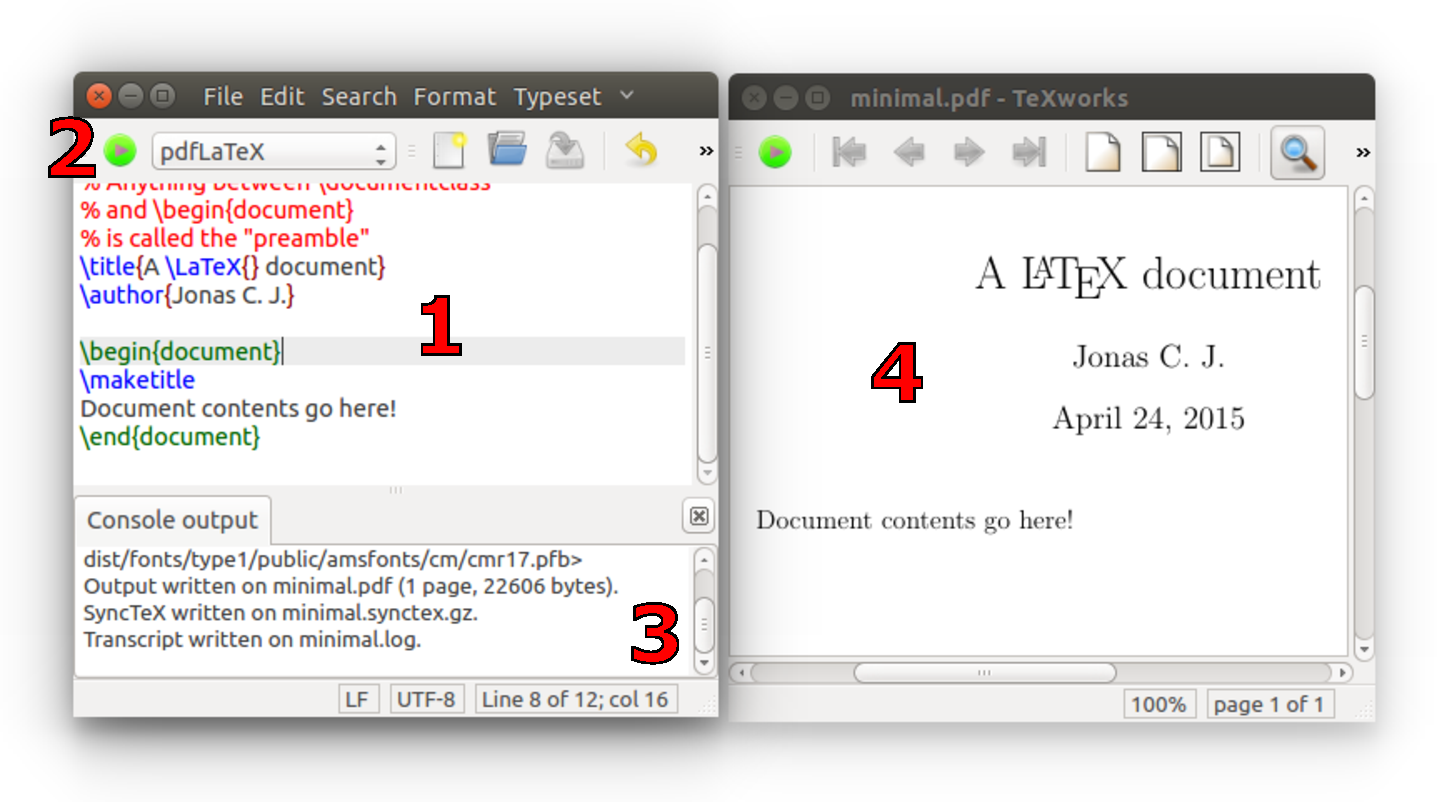
\includegraphics[width=\textwidth]{figs/texworks.pdf}
\end{frame}


% % % % % % Frame % % % % % % 
\begin{frame}[fragile]
\frametitle{How to use \LaTeX{}}
\framesubtitle{TexShop (Mac / OSX)}
\begin{enumerate}
	\item Text input - where you write your \LaTeX{} commands and text.
	\item Typeset-button - click to compile your document.
 	\item Save-dialog - Choose \emph{Unicode (UTF-8)} as encoding.
	\item Built-in document viewer.
	\item Console output - errors, warnings etc. are shown here.
\end{enumerate}

\begin{center}
\includegraphics[width=0.8\textwidth]{figs/texshop.pdf}
\end{center}
\end{frame}

% % % % % % Frame % % % % % % 
\begin{frame}[fragile]
\frametitle{Online \LaTeX{} editors}
\begin{itemize}
	\item For quick and dirty collaboration.
	\item When you urgently need \LaTeX{} on another computer.
	\item Until you get LaTeX working on your own computer.
\end{itemize}
\url{https://www.overleaf.com/}
\\
\\
\url{https://www.sharelatex.com/}

\end{frame}


% % % % % % Frame % % % % % % 
\begin{frame}[fragile]
\frametitle{How to use \LaTeX{}}
\framesubtitle{Command line}
\begin{minted}[linenos]{bash}
jonas@trogdor:/tmp/minimal$ ls
jonas@trogdor:/tmp/minimal$ cat << EOF > minimal.tex
> \documentclass[a4paper, 12pt]{article}
> \title{A \LaTeX{} document}
> \author{Jonas C. J.}
> \begin{document}
> \maketitle
> Document contents go here!
> \end{document}
> EOF
jonas@trogdor:/tmp/minimal$ pdflatex minimal.tex 
This is pdfTeX, Version 3.141 [output truncated]
Transcript written on minimal.log.
jonas@trogdor:/tmp/minimal$ ls
minimal.aux  minimal.log  minimal.pdf  minimal.tex
\end{minted}

\end{frame}


% % % % % % Frame % % % % % % 
\begin{frame}[fragile]
\frametitle{Writing non-ASCII characters}
\begin{columns}
    \begin{column}{.48\textwidth} 
		\latexcode{examples/non-ascii-chars.tex}
	 	\captionof*{lstlisting}{non-ascii-chars.tex}
	\end{column}%
	\begin{column}{.48\textwidth}
		\includegraphics[clip=true, frame, trim=2cm 16.5cm 8cm 5.5cm, width=\textwidth]{examples/non-ascii-chars.pdf}
	 	\captionof*{figure}{PDF output.}
	\end{column}
\end{columns}
\end{frame}


% % % % % % Frame % % % % % % 
\begin{frame}[fragile]
\frametitle{Paragraphs and spacing}
\begin{columns}
    \begin{column}{.48\textwidth} 
		\latexcode[]{examples/paragraphs.tex}
	 	\captionof*{listing}{paragraphs.tex}
	\end{column}%
	\begin{column}{.48\textwidth}
		\includegraphics[clip=true, frame, trim=2cm 12.5cm 8cm 5.5cm, width=\textwidth]{examples/paragraphs.pdf}
	 	\captionof*{figure}{PDF output.}
	\end{column}
\end{columns}
\end{frame}

% % % % % % Frame % % % % % % 
\begin{frame}[fragile]
\frametitle{Sections}
\begin{itemize}
	\item Use sections to give your document structure!
\end{itemize}

\begin{columns}
    \begin{column}{.48\textwidth} 
		\latexcode{examples/sections.tex}
	 	\captionof*{lstlisting}{sections.tex}
	\end{column}%
	\begin{column}{.48\textwidth}
		\includegraphics[clip=true, frame, trim=2cm 14cm 8cm 5.5cm, width=\textwidth]{examples/sections.pdf}
	 	\captionof*{figure}{PDF output.}
	\end{column}
\end{columns}
\end{frame}


% % % % % % Frame % % % % % % 
\begin{frame}[fragile]
\frametitle{Lorem ipsum - placeholder text}
\begin{itemize}
	\item<+-> The \verb!lipsum! package provides filler text.
	\item<+-> It is scrambled Latin, a standard filler text in the typesetting industry (since the 1500's).
	\item<+-> The original first sentence, translated to English, reads: ``Neither is there anyone who loves, pursues or desires pain itself because it is pain".
\end{itemize}

\begin{columns}
    \begin{column}{.48\textwidth} 
		\latexcode[]{examples/lipsum.tex}
	 	\captionof*{listing}{lipsum.tex}
	\end{column}%
	\begin{column}{.48\textwidth}
		\includegraphics[clip=true, frame, trim=2cm 16cm 8cm 5.5cm, width=\textwidth]{examples/lipsum.pdf}
	 	\captionof*{figure}{PDF output.}
	\end{column}
\end{columns}
\end{frame}

% % % % % % Frame % % % % % % 
\begin{frame}[fragile]
\frametitle{Table of contents}
\begin{itemize}
	\item You need to compile twice to get the table of contents.
	\item Shame on any and all \emph{computer scientists} who can not figure out why!
\end{itemize}
\begin{columns}
    \begin{column}{.48\textwidth} 
		\latexcode[firstline=12, lastline=32]{examples/tableofcontents.tex}
	 	\captionof*{lstlisting}{tableofcontents.tex}
	\end{column}%
	\begin{column}{.48\textwidth}
		\includegraphics[page=2,clip=true, frame, trim=2cm 19cm 8cm 2cm, width=\textwidth]{examples/tableofcontents.pdf}
	 	\captionof*{figure}{PDF output.}
	\end{column}
\end{columns}
\end{frame}

% % % % % % Frame % % % % % % 
\begin{frame}
\frametitle{Time for exercises!}
\begin{itemize}
	\item I: Basics
\end{itemize}
\end{frame}

% % % % % % Frame % % % % % % 
\begin{frame}[fragile]
\frametitle{History of \LaTeX{}}
\begin{block}{Mid-Late 1970's}
\emph{Donald Knuth} (mathematician, computer scientist, 1974 Turing Award recipient) is horrified by the typesetting of the 2nd edition of his book \emph{The Art of Computer Programming} , and decides to make his own high quality digital typesetting system.
\end{block}

\begin{columns}
    \begin{column}{.3\textwidth} 
		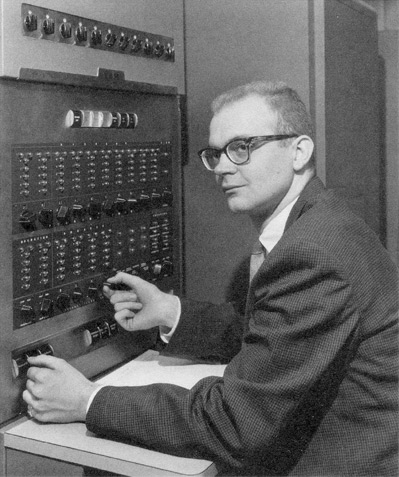
\includegraphics[width=\columnwidth]{figs/young-donald-knuth-ibm-650-1958.jpg}
	 	\captionof*{figure}{D. Knuth, 1958}
	\end{column}%
	\begin{column}{.58\textwidth}
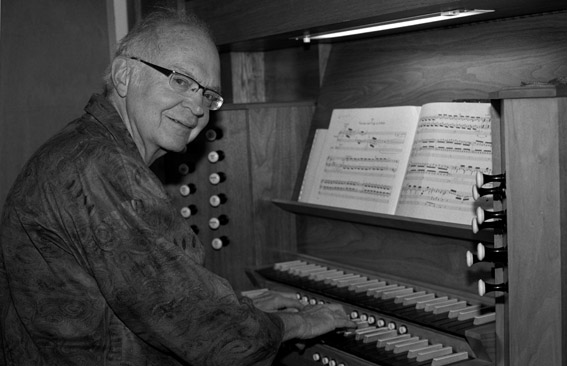
\includegraphics[width=\columnwidth]{figs/dek-badge-20120614.jpg}
	 	\captionof*{figure}{D. Knuth, 2012}
	\end{column}
\end{columns}
\end{frame}

% % % % % % Frame % % % % % % 
\begin{frame}[fragile]
\frametitle{History of \LaTeX{}}
\begin{block}{1978}
Donald Knuth releases \TeX{} typesetting system. The system \LaTeX{} is built on top of.
\end{block}
\pause

\begin{columns}[T]
	\begin{column}{.3\textwidth}
		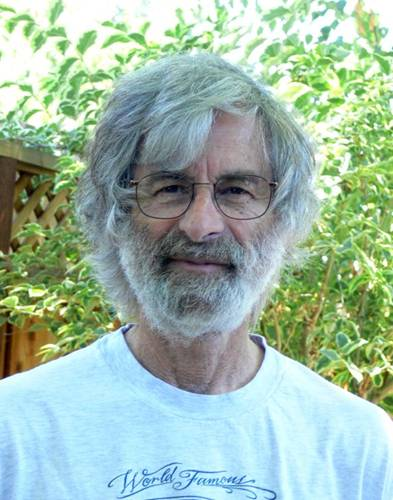
\includegraphics[width=\columnwidth]{figs/lamport.jpg}
			 	\captionof*{figure}{L. Lamport, mid-2000}
	\end{column}
    \begin{column}{.65\textwidth} 
\begin{block}{Early-Mid 1980's}
\emph{Leslie Lamport} (computer scientist, 2013 Turing Award recipient) releases his personal library of \TeX{} macros, and that is the first version of \LaTeX{}, which is short for \emph{Lamport}\TeX{}.
\end{block}    
\pause
\begin{block}{Today}
\LaTeX{} is maintained by volunteers at \url{http://latex-project.org}.
\end{block}

	\end{column}%
\end{columns}

\end{frame}



% % % % % % Frame % % % % % % 
\begin{frame}[fragile]
\frametitle{Become self-sufficient}
\framesubtitle{Use all resources available to you!}
It is very important to learn how to learn more \LaTeX{}, and solve problems you encounter outside of this course. This course only scratches the surface of \LaTeX{}!
\pause

\begin{description}
	\item[``Books'']<+-> The Not So Short Guide to LaTeX (lshort): \url{https://tobi.oetiker.ch/lshort/}

	\item[Web search]<+-> Search for your problem, e.g. ``latex page x of y''
	\item[Wiki's]<+-> \url{http://en.wikibooks.org/wiki/LaTeX/}

	\item[QA sites]<+-> \url{http://tex.stackexchange.com/}

	\item[Chat]<+-> IRC, \#latex @ chat.freenode.net (\url{https://webchat.freenode.net/})
\end{description}

\end{frame}

% % % % % % Frame % % % % % % 
\begin{frame}[fragile]
\frametitle{Become self-sufficient}
\framesubtitle{Look in the log!}

\begin{itemize}
\item Latex produces a log file of what it is doing. Upon errors it will write error messages, and sometimes proposals on how to correct the errors.
\item Find in the the folder next to your \verb!.tex! file.
\item It is called \verb!name-of-your-texfile.log!
\item Your editor might also have a built-in log viewer which highlights errors.
\end{itemize}
\end{frame}


% % % % % % Frame % % % % % % 
\begin{frame}
\frametitle{Time for exercises!}
\begin{itemize}
\item II Towards self-sufficiency
\end{itemize}
\end{frame}



% % % % % % Frame % % % % % % 
\begin{frame}[fragile]
\frametitle{Change locale}
\begin{itemize}
	\item \verb!\usepackage[danish]{babel}! is the standard way of changing language of typographical elements.
\end{itemize}
\begin{columns}
    \begin{column}{.48\textwidth} 
		\latexcode[firstline=8, lastline=32]{examples/babel.tex}
	 	\captionof*{lstlisting}{babel.tex}
	\end{column}%
	\begin{column}{.48\textwidth}
		\includegraphics[page=1,clip=true, frame, trim=2cm 14cm 8cm 6cm, width=\textwidth]{examples/babel.pdf}
	 	\captionof*{figure}{PDF output.}
	\end{column}
\end{columns}
\end{frame}



% % % % % % Frame % % % % % % 
\begin{frame}[fragile]
\frametitle{Enter math mode}
\begin{itemize}
\item Mathematical expressions are typed in math mode.
\end{itemize}
\begin{columns}
    \begin{column}{.48\textwidth} 
		\latexcode[firstline=12, lastline=32]{examples/math1.tex}
	 	\captionof*{lstlisting}{math1.tex}
	\end{column}%
	\begin{column}{.48\textwidth}
		\includegraphics[clip=true, frame, trim=2cm 15cm 8cm 6cm, width=\textwidth]{examples/math1.pdf}
	 	\captionof*{figure}{PDF output.}
	\end{column}
\end{columns}

\end{frame}


% % % % % % Frame % % % % % % 
\begin{frame}[fragile]
\frametitle{Beautiful math}
\emph{Donald Knuth} invented \TeX{} to typeset beautiful math, among other things, let us not misuse his tool!
\begin{columns}
    \begin{column}{.48\textwidth} 
		\latexcode[firstline=10,lastline=32]{examples/math-beautiful.tex}
	 	\captionof*{lstlisting}{math-beautiful.tex}
	\end{column}%
	\begin{column}{.48\textwidth}
		\includegraphics[clip=true, frame, trim=2cm 19cm 8cm 2cm, width=\textwidth]{examples/math-beautiful.pdf}
	 	\captionof*{figure}{PDF output.}
	\end{column}
\end{columns}
\end{frame}

% % % % % % Frame % % % % % % 
\begin{frame}[fragile]
\frametitle{Labels and references}
\begin{columns}
    \begin{column}{.48\textwidth} 
		\latexcode[firstline=13, lastline=32]{examples/ref-label.tex}
	 	\captionof*{lstlisting}{ref-label.tex}
	\end{column}%
	\begin{column}{.48\textwidth}
		\includegraphics[clip=true, frame, trim=3cm 10cm 3cm 5cm, width=\textwidth]{examples/ref-label.pdf}
	 	\captionof*{figure}{PDF output.}
	\end{column}
\end{columns}

\end{frame}

% % % % % % Frame % % % % % % 
\begin{frame}
\frametitle{Custom commands}

\begin{columns}[b]
    \begin{column}{.48\textwidth} 
		\latexcode[firstline=10, lastline=30]{examples/renew-newcommand.tex}
	 	\captionof*{lstlisting}{renew-newcommand.tex}
	\end{column}%
	\begin{column}{.48\textwidth}
		\includegraphics[clip=true, frame, trim=2cm 17cm 6cm 3cm, width=\textwidth]{examples/renew-newcommand.pdf}
	 	\captionof*{figure}{PDF output.}
	\end{column}
\end{columns}
\end{frame}

% % % % % % Frame % % % % % % 
\begin{frame}
\frametitle{Time for exercises!}
\begin{center}
\begin{itemize}
	\item III: Math I
	\item IV: Labels and references
	\item V: Custom commands
\end{itemize}
\end{center}
\end{frame}

% % % % % % Frame % % % % % % 
\begin{frame}
\frametitle{Math - Aligning and numbering equations}
\begin{columns}[b]
    \begin{column}{.48\textwidth} 
		\latexcode[firstline=10, lastline=30]{examples/math-align.tex}
	 	\captionof*{lstlisting}{math-align.tex}
	\end{column}%
	\begin{column}{.48\textwidth}
		\includegraphics[clip=true, frame, trim=2cm 17cm 6cm 3cm, width=\textwidth]{examples/math-align.pdf}
	 	\captionof*{figure}{PDF output.}
	\end{column}
\end{columns}
\end{frame}

% % % % % % Frame % % % % % % 
\begin{frame}
\frametitle{Math - Matrices and cases}
\begin{columns}[b]
    \begin{column}{.48\textwidth} 
		\latexcode[firstline=10, lastline=30]{examples/math-cases-matrix.tex}
	 	\captionof*{lstlisting}{math-cases-matrix.tex}
	\end{column}%
	\begin{column}{.48\textwidth}
		\includegraphics[clip=true, frame, trim=3cm 19cm 7cm 3cm, width=\textwidth]{examples/math-cases-matrix.pdf}
	 	\captionof*{figure}{PDF output.}
	\end{column}
\end{columns}
\end{frame}

% % % % % % Frame % % % % % % 
\begin{frame}
\frametitle{Units}
\begin{columns}[b]
    \begin{column}{.48\textwidth} 
		\latexcode[firstline=10, lastline=30]{examples/units.tex}
	 	\captionof*{lstlisting}{units.tex}
	\end{column}%
	\begin{column}{.48\textwidth}
		\includegraphics[clip=true, frame, trim=2cm 10cm 5cm 4cm, width=\textwidth]{examples/units.pdf}
	 	\captionof*{figure}{PDF output.}
	\end{column}
\end{columns}
\end{frame}


% % % % % % Frame % % % % % % 
\begin{frame}
\frametitle{Lists}
\begin{columns}[b]
    \begin{column}{.48\textwidth} 
		\latexcode[firstline=10, lastline=26]{examples/lists.tex}
	 	\captionof*{lstlisting}{lists.tex}
	\end{column}%
	\begin{column}{.48\textwidth}
		\includegraphics[clip=true, frame, trim=2cm 19cm 8cm 3cm, width=\textwidth]{examples/lists.pdf}
	 	\captionof*{figure}{PDF output.}
	\end{column}
\end{columns}
\end{frame}


% % % % % % Frame % % % % % % 
\begin{frame}
\frametitle{Tabels}
\begin{columns}[b]
    \begin{column}{.48\textwidth} 
		\latexcode[firstline=10, lastline=30]{examples/tables.tex}
	 	\captionof*{lstlisting}{tables.tex}
	\end{column}%
	\begin{column}{.48\textwidth}
		\includegraphics[clip=true, frame, trim=2cm 18cm 6cm 3cm, width=\textwidth]{examples/tables.pdf}
	 	\captionof*{figure}{PDF output.}
	\end{column}
\end{columns}
\end{frame}

% % % % % % Frame % % % % % % 
\begin{frame}
\frametitle{Time for exercises!}
\begin{itemize}
	\item VI: Math II
	\item VII: Units
	\item VIII: Lists
	\item IX: Tables
\end{itemize}
\end{frame}

% % % % % % Frame % % % % % % 
\begin{frame}
\frametitle{Graphics and figures}
\begin{columns}[b]
    \begin{column}{.48\textwidth} 
		\latexcode[firstline=10, lastline=30]{examples/fig.tex}
	 	\captionof*{lstlisting}{fig.tex}
	\end{column}%
	\begin{column}{.48\textwidth}
		\includegraphics[clip=true, frame, trim=3cm 4cm 2.5cm 5cm, width=\textwidth]{examples/fig.pdf}
	 	\captionof*{figure}{PDF output.}
	\end{column}
\end{columns}
\end{frame}

% % % % % % Frame % % % % % % 
\begin{frame}
\frametitle{Subfigures}
\begin{columns}[b]
    \begin{column}{.48\textwidth} 
		\latexcode[firstline=10, lastline=30]{examples/subfig.tex}
	 	\captionof*{lstlisting}{subfig.tex}
	\end{column}%
	\begin{column}{.48\textwidth}
		\includegraphics[clip=true, frame, trim=3cm 6cm 2.5cm 7cm, width=\textwidth]{examples/subfig.pdf}
	 	\captionof*{figure}{PDF output.}
	\end{column}
\end{columns}
\end{frame}


% % % % % % Frame % % % % % % 
\begin{frame}
\frametitle{Digital graphics}

\begin{itemize}
	\item How can we store graphics digitally?
	\item Is there more than one method?
	\item If so, do they have advantages and disadvantages?
\end{itemize}
	\center
		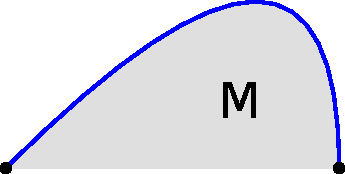
\includegraphics[width=0.8\textwidth]{figs/vector.pdf}
	 	\captionof*{figure}{An illustration / a figure / a schematic / an image.}    
		
\end{frame}


% % % % % % Frame % % % % % % 
\begin{frame}
\frametitle{Digital graphics}

\begin{columns}[t]
    \begin{column}{.48\textwidth} 
	\begin{block}{Bitmap (raster graphics)}
	\begin{equation*}
\begin{bmatrix}
C_{11}  & C_{12} & \cdots & C_{1w} \\
C_{21}  & C_{22} & \cdots & C_{2w} \\
\vdots  & \vdots & \ddots & \vdots \\
C_{h1} & C_{h2} & \cdots & C_{hw}
\end{bmatrix}		
	\end{equation*}
\rawcode{figs/bitmap.txt}	
	\end{block}	 	 	
	\end{column}%
    \begin{column}{.48\textwidth} 
	\begin{block}{Shapes (vector graphics)}
	\xmlcode{figs/vector.svg}
	\end{block} 	 	   	 	
	\end{column}%
\end{columns}

\unfootnote{$00 00 00 04_{16} = 0\cdot16^8 + \ldots + 0\cdot16^1 + 4\cdot16^0 = 4_{10}$}
\end{frame}



% % % % % % Frame % % % % % % 
\begin{frame}
\frametitle{Vector vs. raster graphics}
\begin{itemize}
\item Raster graphics scale poorly (i.e. prints poorly if originally of low resolution)
\item Vector graphics scale to any size without loss of quality
\end{itemize}
\begin{columns}[b]
    \begin{column}{.48\textwidth} 
		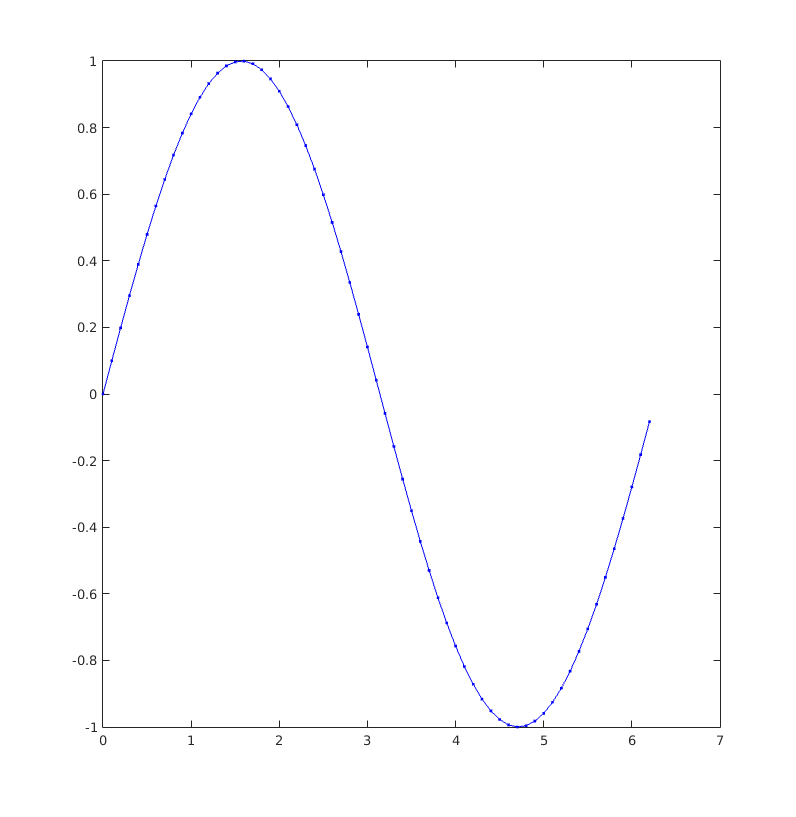
\includegraphics[clip=true,trim=13.5cm 1.8cm 6cm 18.5cm, width=\textwidth]{figs/sine.png}
	 	\captionof*{figure}{Raster graphics.}
	\end{column}%
	\begin{column}{.48\textwidth}
		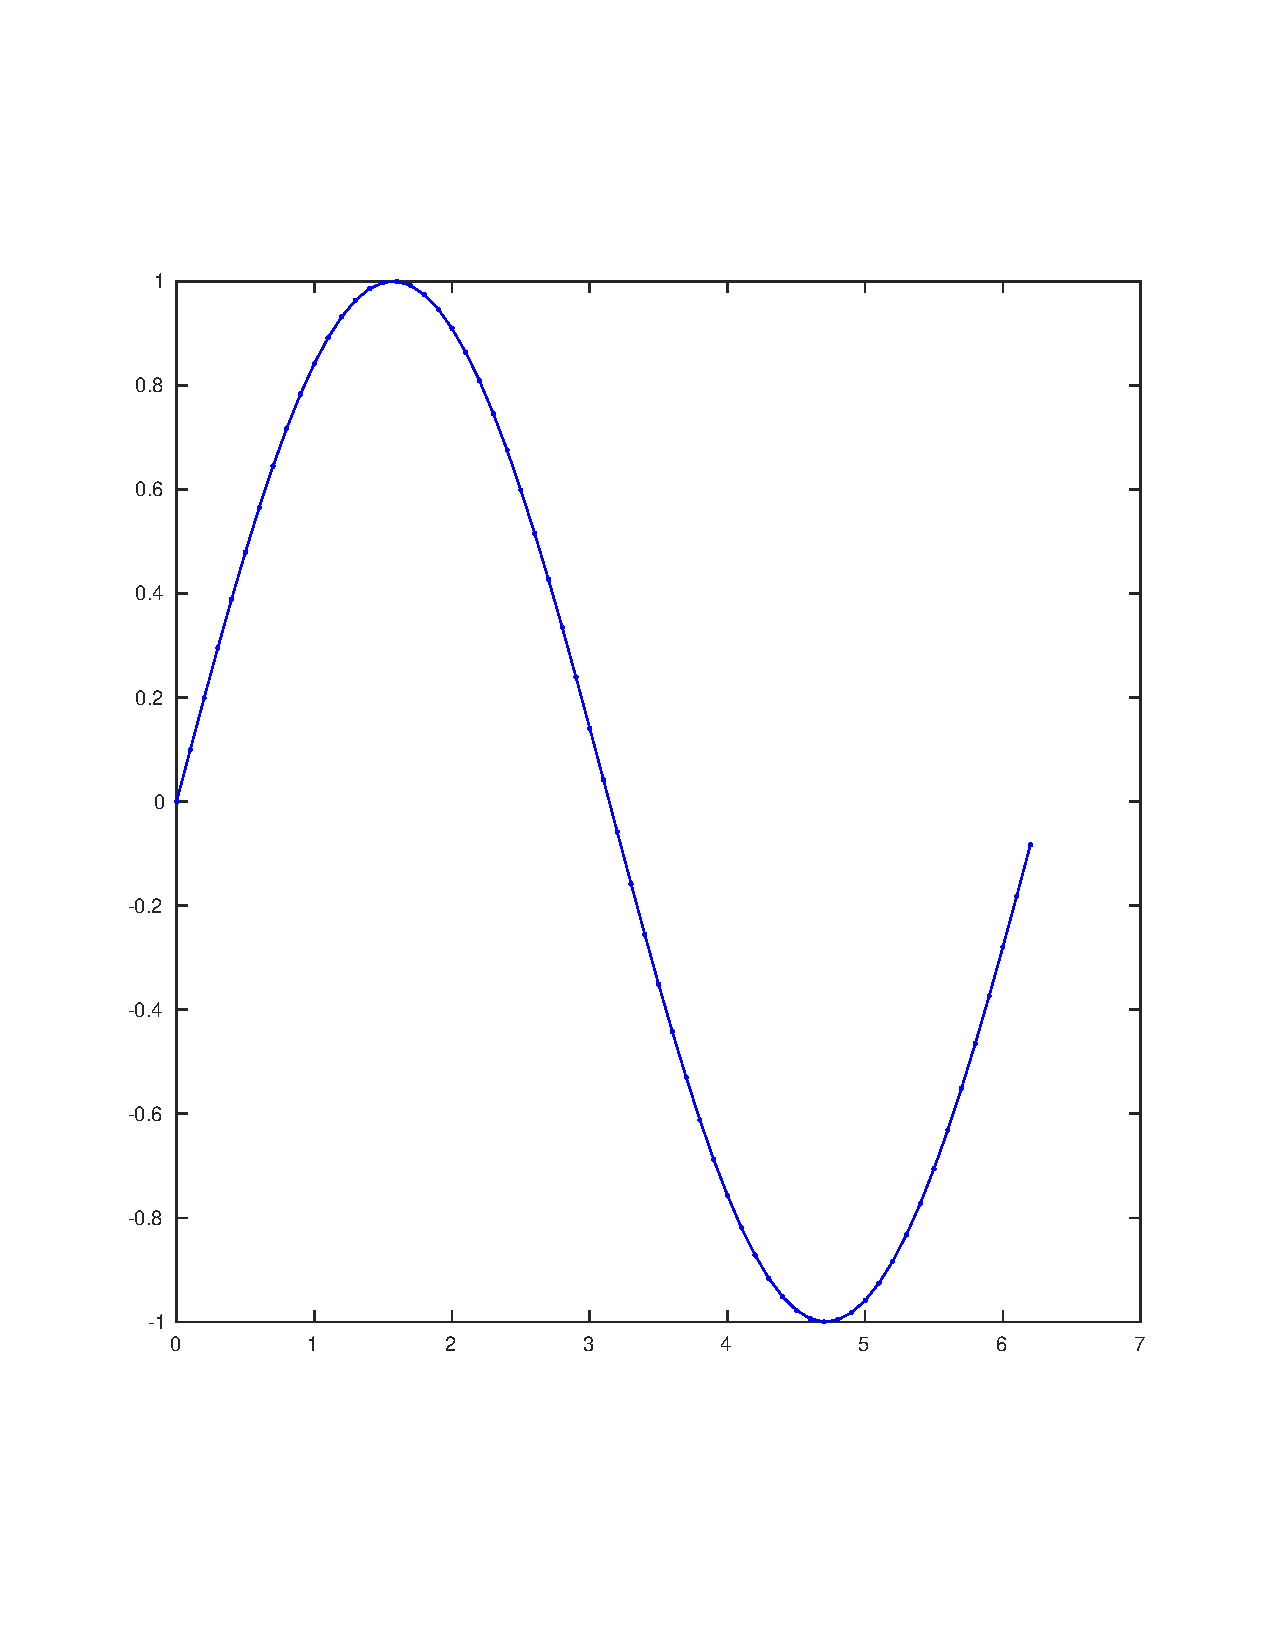
\includegraphics[clip=true, trim=14cm 5cm 6cm 21.5cm, width=\textwidth]{figs/sine.pdf}
	 	\captionof*{figure}{Vector graphics.}
	\end{column}
\end{columns}
\end{frame}

% % % % % % Frame % % % % % % 
\begin{frame}
\frametitle{Raster graphic format}

\begin{columns}[b]
    \begin{column}{.48\textwidth} 
    \center
	 	
\includegraphics[width=0.6\textwidth]{figs/fig_64_32.jpg}
	 	\captionof*{figure}{JPEG 64x32 px}    
		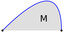
\includegraphics[width=0.6\textwidth]{figs/fig_128_64.jpg}
	 	\captionof*{figure}{JPEG 128x64 px}
	 	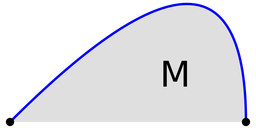
\includegraphics[width=0.6\textwidth]{figs/fig_256_128.jpg}
	 	\captionof*{figure}{JPEG 256x128 px}   	 	
	\end{column}%
    \begin{column}{.48\textwidth} 
    \center
	 	
\includegraphics[width=0.6\textwidth]{figs/fig_64_32.png}
	 	\captionof*{figure}{PNG 64x32 px}    
		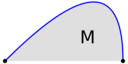
\includegraphics[width=0.6\textwidth]{figs/fig_128_64.png}
	 	\captionof*{figure}{PNG 128x64 px}
	 	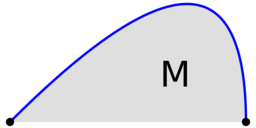
\includegraphics[width=0.6\textwidth]{figs/fig_256_128.png}
	 	\captionof*{figure}{PNG 256x128 px}   	 	
	\end{column}%
\end{columns}
\end{frame}

% % % % % % Frame % % % % % % 
\begin{frame}
\frametitle{Float placement}
\begin{columns}[b]
    \begin{column}{.48\textwidth} 
		\latexcode[firstline=10, lastline=37]{examples/float-placement.tex}
	 	\captionof*{lstlisting}{float-placement.tex}
	\end{column}%
	\begin{column}{.48\textwidth}
		\includegraphics[clip=true, frame, trim=3cm 6cm 2.5cm 5cm, width=\textwidth]{examples/float-placement.pdf}
	 	\captionof*{figure}{PDF output.}
	\end{column}
\end{columns}
\end{frame}




% % % % % % Frame % % % % % % 
\begin{frame}
\frametitle{Bibliography with Bib\TeX{}}
Compile like this when first inserting the bibliography, or later whenever you change it:

PDFLaTeX >> BibTeX >> PDFLaTeX >> PDFLaTeX\\

\begin{columns}[b]
    \begin{column}{.48\textwidth} 
		\latexcode[firstline=10, lastline=16]{examples/bibtex.tex}
	 	\captionof*{lstlisting}{bibtex.tex}
	 	\latexcode{examples/refs.bib}
	 	\captionof*{lstlisting}{refs.bib}
	\end{column}%
	\begin{column}{.48\textwidth}
		\includegraphics[clip=true, frame, trim=2cm 19cm 8cm 3cm, width=\textwidth]{examples/bibtex.pdf}
	 	\captionof*{figure}{PDF output.}
	\end{column}
\end{columns}
\end{frame}


% % % % % % Frame % % % % % % 
\begin{frame}
\frametitle{Bibliography}
\framesubtitle{Reference types and bibliography styles}

\begin{block}{Reference types}
\url{http://en.wikibooks.org/wiki/LaTeX/Bibliography_Management\#Standard_templates}
\end{block}

\begin{block}{Bibliography styles}
\url{https://www.sharelatex.com/learn/Bibtex_bibliography_styles}
\end{block}

\end{frame}

% % % % % % Frame % % % % % % 
\begin{frame}
\frametitle{Include code in \LaTeX}
\framesubtitle{Poor man's solution: listings-package}
\begin{columns}[b]
    \begin{column}{.48\textwidth} 
		\latexcode[firstline=7, lastline=29]{examples/listings1.tex}
	 	\captionof*{lstlisting}{listings1.tex}
	\end{column}%
	\begin{column}{.48\textwidth}
		\includegraphics[clip=true, frame, trim=3cm 20cm 7cm 3cm, width=\textwidth]{examples/listings1.pdf}
	 	\captionof*{figure}{PDF output.}
	\end{column}
\end{columns}
\end{frame}

% % % % % % Frame % % % % % % 
\begin{frame}
\frametitle{Include code in \LaTeX}
\framesubtitle{Poor man's solution: listings-package}
\begin{columns}[b]
    \begin{column}{.48\textwidth} 
		\latexcode[firstline=7, lastline=29]{examples/listings2.tex}
	 	\captionof*{lstlisting}{listings2.tex}
	\end{column}%
	\begin{column}{.48\textwidth}
		\includegraphics[clip=true, frame, trim=3cm 12cm 5cm 3cm, width=\textwidth]{examples/listings2.pdf}
	 	\captionof*{figure}{PDF output.}
	\end{column}
\end{columns}
\end{frame}

% % % % % % Frame % % % % % % 
\begin{frame}
\frametitle{Include code in \LaTeX}
\framesubtitle{minted-package}
\begin{columns}[b]
    \begin{column}{.48\textwidth} 
		\latexcode[firstline=7, lastline=25]{examples/minted1.tex}
	 	\captionof*{lstlisting}{minted1.tex}
	\end{column}%
	\begin{column}{.48\textwidth}
		\includegraphics[clip=true, frame, trim=2cm 15cm 6cm 3cm, width=\textwidth]{examples/minted1.pdf}
	 	\captionof*{figure}{PDF output.}
	\end{column}
\end{columns}
\end{frame}

% % % % % % Frame % % % % % % 
\begin{frame}
\frametitle{Include code in \LaTeX}
\framesubtitle{minted-package}
\begin{columns}[b]
    \begin{column}{.48\textwidth} 
		\latexcode[firstline=7, lastline=25]{examples/minted2.tex}
	 	\captionof*{lstlisting}{minted2.tex}
	\end{column}%
	\begin{column}{.48\textwidth}
		\includegraphics[clip=true, frame, trim=2cm 11cm 6cm 3cm, width=\textwidth]{examples/minted2.pdf}
	 	\captionof*{figure}{PDF output.}
	\end{column}
\end{columns}
\end{frame}


% % % % % % Frame % % % % % % 
\begin{frame}
\frametitle{Source code}
sudo apt-get install python-pygments
sudo apt-get install python-pip \&\& sudo pip install pygments
check: pygmentize -L lexers
Texworks > Edit > Preferences > Typesetting > 1
\end{frame}

% % % % % % Frame % % % % % % 
\begin{frame}
\frametitle{Include code in \LaTeX}
\framesubtitle{listings vs. minted}
\begin{columns}[t]
    \begin{column}{.48\textwidth} 
	\begin{block}{listings-package}
	Pros:
	\begin{itemize}
		\item Works out of the box (just load the package)
	\end{itemize}
	Cons:
	\begin{itemize}
		\item Limited highlighting capabilities.
		\item Confusing syntax
	\end{itemize}
	\end{block}
	\end{column}	
	
    \begin{column}{.48\textwidth} 
	\begin{block}{minted-package}
	Pros:
	\begin{itemize}
		\item Superior highlighting capabilities
		\item Better syntax
	\end{itemize}
	Cons:
	\begin{itemize}
		\item Requires additional setup (python, python-pygments and shell access).
	\end{itemize}
	\end{block}
	\end{column}
\end{columns}

\end{frame}


% % % % % % Frame % % % % % % 
\begin{frame}
\frametitle{TODO before 2016}
\begin{itemize}
	\item Fortæl om b,t,h,h! og H ved figurer og tabeller.
	\item Bedre gennemgang af bibtex. Fokus på at det er to filer, og hvordan man compiler.
	\item En øvelse mere i at finde ud af ting selv. Table of cntent på sin egen side dur ikke fordi du har vist det i et eksempel.
\end{itemize}
\end{frame}

\end{document}


